\chapter{Conoscenza di dominio}
\label{sec:domain-knowledge}

La comprensione del processo produttivo richiede di chiarire il rapporto tra la domanda commerciale, gli ordini che ne organizzano la produzione e le attività attraversate dal materiale. Questo capitolo presenta i concetti e la terminologia utilizzati nel report, a partire dalla documentazione aziendale e dai chiarimenti raccolti durante il progetto.

\section{Ordini di vendita e ordini di produzione}
\label{sec:odv-odp}

Un \textbf{ordine di vendita (ODV)} formalizza la richiesta di fornitura di un cliente e ne definisce le condizioni commerciali. Comprende una o più posizioni.

Una \textbf{posizione ODV} è una singola voce dell'ordine di vendita e descrive una fornitura attraverso le caratteristiche del prodotto, la quantità richiesta e le condizioni di consegna. È identificata dalla coppia numero ODV e numero di posizione e costituisce l'unità di domanda alla quale viene associata la produzione.

Un \textbf{ordine di produzione (ODP)} è la richiesta interna di produrre una determinata quantità di materiale secondo le specifiche assegnate. Costituisce il riferimento per organizzare e registrare le lavorazioni. Ogni ODP appartiene a una sola posizione ODV, la cui produzione può essere ripartita tra uno o più ODP.

% Cardinalities: notes/Meeting September 29 2026 Decisions.md and current raw data.
% The August email's one-to-one statement does not support these cardinalities.
La \cref{fig:order-hierarchy} riassume le relazioni tra le tre entità, distinguendo il lato commerciale da quello produttivo.

\begin{figure}[htbp]
\centering
\reportfigurecontent{% Schema concettuale: le cardinalità non rappresentano conteggi di un caso reale.
\begin{tikzpicture}[
  scale=0.8,transform shape,
  entity/.style={draw=ReportBlue!45,fill=white,rounded corners=2mm,
    text width=3.6cm,align=center,minimum height=17mm,inner sep=5pt,font=\small},
  relation/.style={-{Stealth[length=2mm]},draw=ReportBlue,line width=0.7pt},
  cardinality/.style={font=\small,text=ReportBlue,fill=white,inner sep=2pt,above=3pt},
  grouplabel/.style={font=\small\bfseries,text=ReportBlue}
]
% Fondi tenui, disegnati prima dei nodi e dei collegamenti.
\path[draw=ReportBlue!35,fill=ReportBlue!7,rounded corners=2mm]
  (-2.3,-1.18) rectangle (7.8,1.18);
\path[draw=ReportAccent!45,fill=ReportAccent!9,rounded corners=2mm]
  (9.8,-1.18) rectangle (14.4,1.18);
\node[grouplabel] at (2.75,1.55) {Lato cliente};
\node[grouplabel,text=ReportAccent!80!black] at (12.1,1.55) {Lato produzione};
\node[entity] (odv) at (0,0) {\textbf{ODV}\\Ordine commerciale};
\node[entity] (position) at (5.5,0) {\textbf{Posizione ODV}\\Singola fornitura};
\node[entity] (odp) at (12.1,0) {\textbf{ODP}\\Ordine di produzione};
\draw[relation] (odv.east) -- node[cardinality,fill=ReportBlue!7] {$1:N$} (position.west);
\draw[relation] (position.east) -- node[cardinality] {$1:N$} (odp.west);
\end{tikzpicture}
}
\caption{Relazioni tra ordine di vendita, posizione ODV e ordine di produzione. Le cardinalità indicano relazioni uno-a-molti.}
\label{fig:order-hierarchy}
\end{figure}

% Example verified directly against all three CSVs in
% StrategicPlannerBeanTech/data/raw/2026-09-24/:
% ordini_di_vendita_260915.csv: Numero_OdV=0001118887, exactly two positions.
% Posizione_OdV=000020: Materiale=3002629, Qta_OdV=40000.
% Posizione_OdV=000030: Materiale=3000022, Qta_OdV=170000.
% ordini_di_produzione_260915.csv, joining on ODV and POSIZIONE_ODV:
% 000020 -> ODP 000010862043 (COD_MATERIALE=3002629).
% 000030 -> ODP 000010865639 and 000010867470 (COD_MATERIALE=3000022).
% ODP identifiers deduplicated before counting; all three have records in
% Consuntivi_260915.csv. Preserve leading zeros in every identifier.
\begingroup
\tcbset{lines before break=12}
\begin{examplebox}[ex:odv-two-odp]{Un ODV con due posizioni e tre ODP}
L'esempio mostra un ordine di vendita articolato in due posizioni, riferite a materiali diversi. Alla prima è associato un solo ordine di produzione, mentre alla seconda ne sono associati due, come illustrato nello schema seguente.

\begin{center}
% Esempio reale: ODV 0001118887; fonti e verifica nel testo della sezione 2.1.
\begin{tikzpicture}[
  every node/.style={font=\small,align=center,inner sep=4pt},
  branch/.style={draw=ReportExample!55!black,line width=0.65pt}
]
\node (odv) at (0,0) {\textbf{ODV}\\\texttt{0001118887}};
\node (posone) at (4.25,0.9) {\textbf{Posizione} \texttt{000020}\\Materiale \texttt{3002629}};
\node (postwo) at (4.25,-0.9) {\textbf{Posizione} \texttt{000030}\\Materiale \texttt{3000022}};
\node (odpfirst) at (9,0.9) {\textbf{ODP} \texttt{000010862043}};
\node (odpsecond) at (9,-0.5) {\textbf{ODP} \texttt{000010865639}};
\node (odpthird) at (9,-1.3) {\textbf{ODP} \texttt{000010867470}};
\draw[branch] (odv.east) -- (1.8,0);
\draw[branch] (posone.west) -- (1.8,0.9) -- (1.8,-0.9) -- (postwo.west);
\draw[branch] (posone.east) -- (odpfirst.west);
\draw[branch] (postwo.east) -- (6.65,-0.9);
\draw[branch] (odpsecond.west) -- (6.65,-0.5) -- (6.65,-1.3) -- (odpthird.west);
\end{tikzpicture}

\end{center}
\end{examplebox}
\endgroup

\section{Macrofasi del processo produttivo}
\label{sec:production-phases}

Per realizzare il prodotto richiesto da un ODP, il materiale attraversa un percorso di lavorazioni e controlli, fino al completamento della produzione. Le registrazioni che documentano quanto avvenuto durante questo percorso sono dette \textbf{consuntivi di produzione}. Esse associano all'ODP le attività e gli stati registrati, con le relative informazioni temporali e quantitative, e permettono di ricostruirne la storia produttiva.

Una \textbf{macrofase} è un passaggio di questo percorso, descritto a un livello che riassume il dettaglio delle singole operazioni. Può riunire più lavorazioni in un'unica fase, identificare un controllo oppure rappresentare uno stato del materiale, come l'attesa di un esito o il completamento della produzione. Il termine indica quindi il ruolo del passaggio nel processo e non implica che esso corrisponda a una sola macchina.

Nei consuntivi, ogni registrazione riferita a una macrofase ne descrive una specifica occorrenza per un ODP. Una stessa macrofase può comparire più volte nel percorso dello stesso ordine. I passaggi registrati e le loro relazioni descrivono il \textbf{ciclo produttivo osservato} dell'ODP.

% Inventory checked directly against all records in
% StrategicPlannerBeanTech/data/raw/2026-09-24/Consuntivi_260915.csv,
% field MACHINE_AGGREGATION_CODE: 14 distinct values, 35893 records.
% Counts refer to the final source files before physical-consistency filtering.
% Domain sources:
% - data/raw/2026-09-24/ABS_Flussi_Luna.pptx, slides 1--8;
% - notes/Email Correspondence August 24-26 2026.md;
% - notes/Meeting August 27 2026 Summary.md;
% - notes/Meeting September 29 2026 Decisions.md.
Nei consuntivi sono presenti 14 macrofasi distinte. Il loro significato è ricostruito a partire dal documento aziendale \texttt{ABS\_Flussi\_Luna.pptx} e dalle note di progetto.

Le macrofasi sono raggruppate per funzione in sette categorie: processo iniziale aggregato, lavorazioni meccaniche, trattamenti termici, controlli qualità, confezionamento, attesa e rilascio qualitativo, stati di approntamento.

\subsection{Processo iniziale aggregato}

\begin{description}
\item[\texttt{TRENOLUNA}] Riunisce le attività iniziali in continuo, dal riscaldo al controllo qualità in linea. Nella presentazione queste comprendono la laminazione, seguita dal raffreddamento in placca (\texttt{PLA}) oppure dal passaggio nel forno \texttt{ONA} e dal controllo in linea. Per i bordioni, il percorso comprende invece laminazione e avvolgimento. Nei consuntivi tali attività sono aggregate in un’unica macrofase.
\end{description}

\subsection{Lavorazioni meccaniche}

\begin{description}
\item[\texttt{TAG}] Indica il taglio del materiale mediante seghetti, presente nei percorsi di recupero.

\item[\texttt{MOL}] Indica la molatura del materiale, presente nei percorsi di recupero prima di un nuovo controllo ai banchi.

\item[\texttt{RADDR}] Indica la raddrizzatura, destinata a correggere la rettilineità del materiale. Può essere prevista dopo un trattamento termico oppure come intervento di recupero.
\end{description}

\subsection{Trattamenti termici}

\begin{description}
\item[\texttt{TRATT\_LUNA}] Riunisce i trattamenti a induzione della linea Luna: rinvenimento, normalizzazione e ciclo completo di tempra e rinvenimento. Nella presentazione queste modalità utilizzano la stessa risorsa, mentre nei consuntivi confluiscono in un'unica macrofase.

\item[\texttt{TRATT\_LFC}] Indica il trattamento termico svolto presso un impianto esterno alla linea Luna. Nel progetto questa macrofase è associata alla voce \texttt{DFO} della presentazione. Il termine esterno si riferisce alla linea produttiva e non implica che il trattamento sia affidato a un'altra azienda.
\end{description}

\subsection{Controlli qualità}

\begin{description}
\item[\texttt{BANCHI}] Indica il controllo ai banchi, rappresentati dalla voce banco/metalloscopio. Serve a verificare il materiale e a indirizzare gli eventuali interventi di recupero. È previsto anche un nuovo passaggio ai banchi dopo la molatura.

\item[\texttt{ANTIMIX}] Indica il controllo volto a rilevare mescolamenti qualitativi. Chiude il blocco di recupero e compare anche dopo i trattamenti termici. Il materiale prosegue poi verso i controlli, i trattamenti o il completamento previsti dal percorso.

\item[\texttt{CIRCO}] Indica il controllo mediante \emph{CIRCOGRAPH}, descritto nella presentazione come controllo qualità finale per le rilavorazioni. Compare anche nei percorsi successivi ai trattamenti termici.
\end{description}

\subsection{Confezionamento}

\begin{description}
\item[\texttt{CONF}] Indica il confezionamento del materiale, rappresentato dalla voce \emph{Confez} nella presentazione. È distinto dall'approntamento, che ne registra lo stato di completamento produttivo.
\end{description}

\subsection{Attesa e rilascio qualitativo}

\begin{description}
\item[\texttt{HPT}] Rappresenta l'attesa dell'esito del controllo qualità fuori linea, svolto in laboratorio dopo un trattamento termico. In base al percorso, l'esito consente il rilascio del materiale oppure determina il trattamento successivo.
\end{description}

\subsection{Stati di approntamento}

Le macrofasi \texttt{PRONTO}, \texttt{PRONTO\_QS} e \texttt{PRONTO\_QWR} indicano l'approntamento del materiale al termine del percorso produttivo, senza attestare l'avvenuta spedizione al cliente. Nella presentazione compare la voce \texttt{USCITA}, ricondotta a questi stati senza distinguerne le varianti. Il significato dei suffissi \texttt{QS} e \texttt{QWR} non è specificato nella documentazione disponibile.

\section{Struttura dei cicli produttivi}
\label{sec:base-production-cycles}

Un ciclo produttivo descrive le lavorazioni, i controlli e gli stati attraversati dal materiale e le relazioni tra questi passaggi. Può comprendere diramazioni e ricongiungimenti, anche relativi a porzioni diverse del materiale. Il percorso dipende dalle caratteristiche del prodotto e dagli esiti dei controlli, che possono richiedere rilavorazioni o ulteriori trattamenti anche su una parte del materiale. La presentazione \texttt{ABS\_Flussi\_Luna.pptx} illustra alcuni percorsi possibili e le relative diramazioni, senza costituire un elenco necessariamente esaustivo. Il ciclo di base comprende i passaggi previsti per ottenere il prodotto richiesto. Le rilavorazioni sono gli interventi di recupero che possono aggiungersi a questo percorso.

La \cref{fig:documented-production-graph} sintetizza i percorsi documentati in un unico grafo, accorpando i passaggi comuni. Non tutte le combinazioni di collegamenti sono ammesse per ogni prodotto: valgono le condizioni sui flussi e sugli esiti dei controlli descritte nel testo. I collegamenti che saltano nodi rappresentano sia passaggi opzionali sia differenze tra percorsi. Per esempio, il flusso PLA trattato non include l'\texttt{HPT} iniziale previsto nei flussi ONA trattati.

\begin{sidewaysfigure}[p]
\centering
\resizebox{0.93\linewidth}{!}{% Il PDF vettoriale è generato dal sorgente .dot omonimo.
% Ogni freccia termina sul bordo di un nodo visibile.
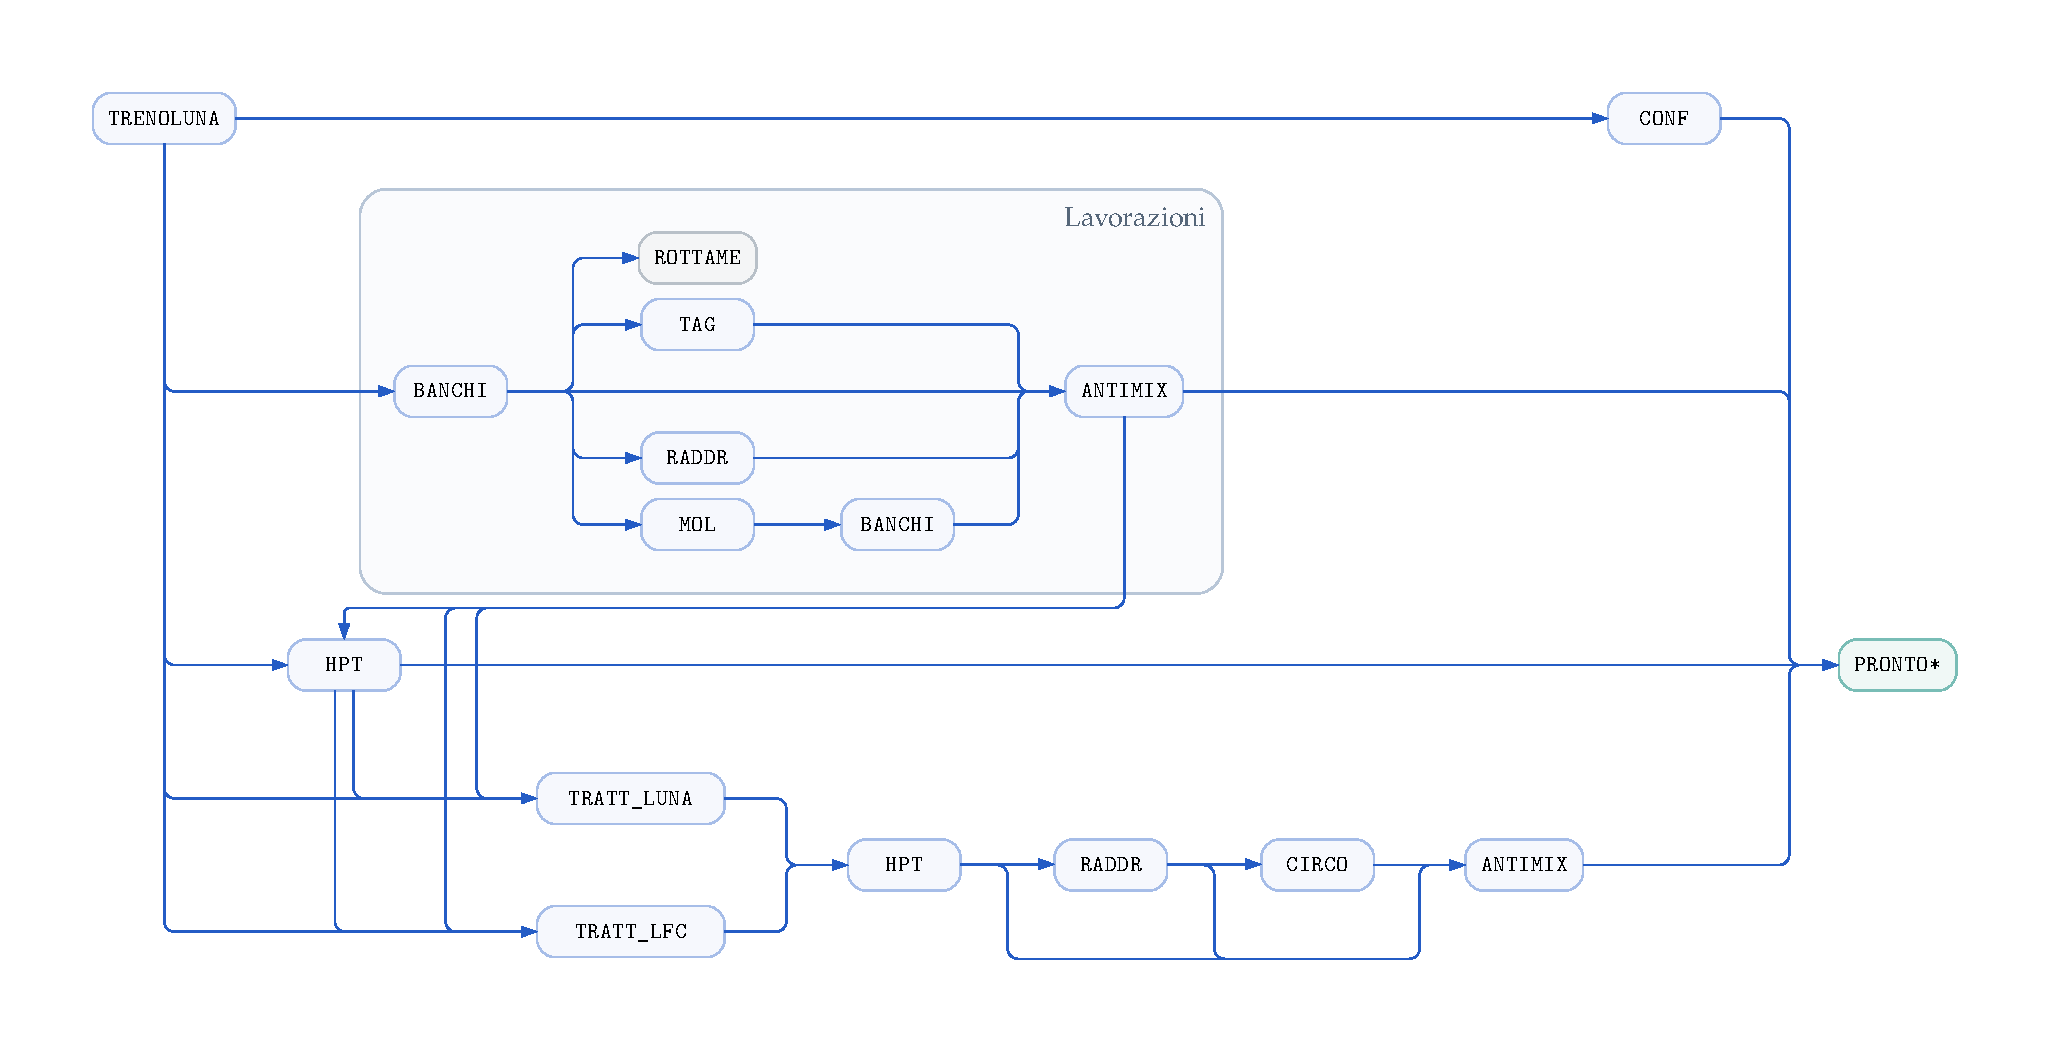
\includegraphics[width=29cm]{figures/documented-production-graph.pdf}
}
\caption{Grafo unico dei percorsi documentati in \texttt{ABS\_Flussi\_Luna.pptx}. \texttt{PRONTO*} riunisce i tre stati di approntamento.}
\label{fig:documented-production-graph}
\end{sidewaysfigure}

% Fonti: ABS_Flussi_Luna.pptx, slide 2--8; trascrizione verificata in
% StrategicPlannerBeanTech/data/raw/2026-09-24/ABS_Flussi_Luna.md.
% Le corrispondenze con le macrofasi sono definite nella sezione 2.2.
\subsection{Percorsi documentati}

Nella presentazione, il \textbf{flusso naturale} porta il materiale conforme al controllo in linea verso il confezionamento e l'approntamento. Il \textbf{flusso bordioni} prevede anch'esso confezionamento e uscita, dopo il passaggio agli avvolgitori. Pur avendo attività iniziali diverse, entrambi sono rappresentati dalla successione \texttt{TRENOLUNA} $\rightarrow$ \texttt{CONF} $\rightarrow$ \texttt{PRONTO*}, dove \texttt{PRONTO*} indica uno dei tre stati di approntamento.

Nel \textbf{flusso ONA}, dopo il processo iniziale è previsto il controllo di laboratorio. Se l'esito è favorevole, il percorso prosegue verso l'approntamento secondo la successione \texttt{TRENOLUNA} $\rightarrow$ \texttt{HPT} $\rightarrow$ \texttt{PRONTO*}. Un esito non conforme può richiedere un ulteriore trattamento, seguito da un nuovo controllo e dai passaggi di rilascio previsti.

I \textbf{flussi ONA con trattamento a induzione} comprendono un primo \texttt{HPT}, il trattamento \texttt{TRATT\_LUNA} e un secondo \texttt{HPT}. Nel percorso con rinvenimento segue \texttt{ANTIMIX}. Nel percorso con ciclo completo sono previsti anche \texttt{RADDR} e \texttt{CIRCO}, prima di \texttt{ANTIMIX} e dell'approntamento. Il diagramma con rinvenimento mostra inoltre una continuazione alternativa con ciclo completo, in funzione dell'esito del controllo.

Nel \textbf{flusso PLA con trattamento a induzione}, al processo iniziale seguono \texttt{TRATT\_LUNA}, \texttt{HPT}, \texttt{RADDR}, \texttt{CIRCO} e \texttt{ANTIMIX}, fino all'approntamento. Rispetto ai flussi ONA trattati, non compare il controllo \texttt{HPT} precedente al trattamento.

Nel \textbf{flusso PLA con ricottura esterna}, il trattamento è invece \texttt{TRATT\_LFC}. Seguono \texttt{HPT}, \texttt{RADDR} e \texttt{ANTIMIX}, prima dell'approntamento. Il passaggio intermedio attraverso \texttt{CIRCO} è opzionale. I percorsi descritti possono inoltre comprendere il blocco di rilavorazioni illustrato di seguito.

\subsection{Controlli e rilavorazioni}

Un esito non conforme del controllo in linea può indirizzare parte del materiale verso il blocco di rilavorazioni, che inizia con \texttt{BANCHI}. Da qui sono previsti il passaggio diretto ad \texttt{ANTIMIX} oppure i rami con \texttt{TAG}, \texttt{RADDR} o \texttt{MOL}. Il blocco è indicato come «Lavorazioni» nel grafo. Dopo \texttt{MOL} è obbligatorio un nuovo passaggio a \texttt{BANCHI}, prima di \texttt{ANTIMIX}. Il materiale non recuperabile può invece essere destinato a rottame, che costituisce un'uscita dal flusso utile e non una macrofase presente nei consuntivi.

Nella rappresentazione adottata si ammette che i rami del blocco interessino porzioni diverse del materiale, anche in parallelo. È un'ipotesi di ricostruzione, non una simultaneità attestata dalla presentazione. I percorsi di recupero che proseguono terminano in \texttt{ANTIMIX}, per poi ricongiungersi alla continuazione prevista dal flusso di appartenenza.

Anche l'esito di \texttt{HPT} può modificare il percorso. Nel flusso ONA, il diagramma prevede ulteriori trattamenti mediante \texttt{TRATT\_LFC} o \texttt{TRATT\_LUNA}, ai quali si applica la stessa ipotesi di ripartizione del materiale. Dopo il trattamento è previsto un nuovo \texttt{HPT}, seguito da \texttt{ANTIMIX}, con \texttt{RADDR} opzionale nel ramo indicato.

\subsection{Percorsi documentati e cicli osservati}

La presentazione descrive percorsi tecnologici possibili, mentre i consuntivi riportano le attività registrate per ciascun ODP. Le due rappresentazioni hanno un livello di dettaglio diverso: più attività possono essere aggregate in una macrofase e una stessa macrofase può comparire più volte. L'assenza di un passaggio nei consuntivi non dimostra, da sola, che l'attività non sia avvenuta. Analogamente, un percorso non rappresentato nella presentazione non è necessariamente impossibile.

% Esempio verificato nei CSV Consuntivi_260915.csv e
% ordini_di_produzione_260915.csv, in data/raw/2026-09-24/.
% ODP 000010859984: TRENOLUNA > PRONTO;
% ODV=0007001624, POSIZIONE_ODV=000010.
% ODP 000010858580: TRENOLUNA > BANCHI > ANTIMIX > PRONTO;
% ODV=0001117836, POSIZIONE_ODV=000020.
% Entrambi: PRODOTTO=LAMINATO BARRE, FINITURA=GREZZO, STATO_FISICO=NATURALE.
% CONF non è presente nei record grezzi di entrambi gli ODP.
\begin{examplebox}[ex:base-cycle-and-variant]{Due percorsi osservati per prodotti dello stesso tipo}
Due ODP relativi a laminato barre grezzo allo stato naturale presentano percorsi diversi: il primo riporta soltanto il processo iniziale e l'approntamento, il secondo include anche i controlli ai banchi e all'antimix.

\begin{center}
\begin{tikzpicture}[
  every node/.style={font=\small,inner sep=3pt},
  route/.style={-{Stealth[length=1.5mm]},draw=ReportExample!55!black,line width=0.6pt}
]
\node[anchor=east] at (-1.2,0) {\texttt{000010859984}};
\node (firstin) at (1.1,0) {\texttt{TRENOLUNA}};
\productionstart[route]{firstin}
\node (firstout) at (8.2,0) {\texttt{PRONTO}};
\draw[route] (firstin) -- (firstout);
\node[anchor=east] at (-1.2,-0.8) {\texttt{000010858580}};
\node (secondin) at (1.1,-0.8) {\texttt{TRENOLUNA}};
\productionstart[route]{secondin}
\node (banchi) at (3.6,-0.8) {\texttt{BANCHI}};
\node (antimix) at (5.9,-0.8) {\texttt{ANTIMIX}};
\node (secondout) at (8.2,-0.8) {\texttt{PRONTO}};
\draw[route] (secondin) -- (banchi);
\draw[route] (banchi) -- (antimix);
\draw[route] (antimix) -- (secondout);
\end{tikzpicture}
\end{center}

Il primo percorso coincide con il ciclo di base descritto nella corrispondenza aziendale per il laminato grezzo naturale. La presentazione include invece \texttt{CONF}, la cui registrazione è indicata come discontinua nei chiarimenti aziendali. La sua assenza non basta quindi a identificare una lacuna del ciclo. Il secondo ODP segue il percorso di recupero diretto attraverso i controlli.
\end{examplebox}
